\documentclass[12pt]{article}
% pre\'ambulo

\usepackage{lmodern}
\usepackage[T1]{fontenc}
\usepackage[spanish,activeacute]{babel}
\usepackage{mathtools}
\usepackage{titlesec}
\usepackage{verbatim}
\usepackage{moreverb}
\usepackage{fancybox}
\usepackage{fancyhdr}
\usepackage{graphicx}
\usepackage{array}
\usepackage{enumerate}
\usepackage{multicol}
\usepackage{multirow}
\usepackage[dvipsnames]{xcolor}
\usepackage{amsfonts}
\usepackage{ulem}
\usepackage{array}
\usepackage[utf8]{inputenc}
%\usepackage[usenames]{color}

\newtheorem{defin}{Definición}

%% Figuras
\graphicspath{{./img/}}

\setlength{\textwidth}{18cm}   
\setlength{\evensidemargin}{0.5cm}
\setlength{\footskip}{1.5cm}
\setlength{\textheight}{22cm} 
\voffset -2cm
\hoffset -2cm
\pagestyle{plain}


\begin{document}
	
	
	\decimalpoint
	
	\renewcommand{\tablename}{Tabla}
	
	\fancyput(8.29cm,-11.436cm){
		\setlength{\unitlength}{1in}\hspace{-0.2cm}\fancyoval(7.7,10.4)}
	\thispagestyle{empty}
	\vspace*{\fill}
	\begin{center}
		{\huge Tarea 3. Asistencia a Webinar.} \\\vspace{0.7cm}
		{\huge Aplicaciones del metaverso para la educación basada en simulación
	}\\\vspace{2cm} 
		{\Large por:}	\\\vspace{1cm} 
		{\Large Luis Antonio Fernández Barbosa\\}
		\vspace{6cm} 
	Profesor:\\
	Dr. José Daniel Castro Díaz
		
		
		
	\end{center}
	
	
	\vspace*{\fill}	
	
	\newpage
	\setcounter{page}{1}
	
	\newpage
	
	\section{Introducción}
En la conferencia correspondiente se nos dio a conocer las actualizaciones tecnológicas sobre el metaverso y como se ha empezado a aplicar en la rama de educación médica, muchos asocian al metaverso más como un entretenimiento; así han comenzado a darlo a conocer, sin embargo, ese mundo virtual nos proporciona grandes avances para cualquier rama de investigación y desarrollo (figura \ref{img_2}). 

 	\begin{figure}[h]
 	\centering
 	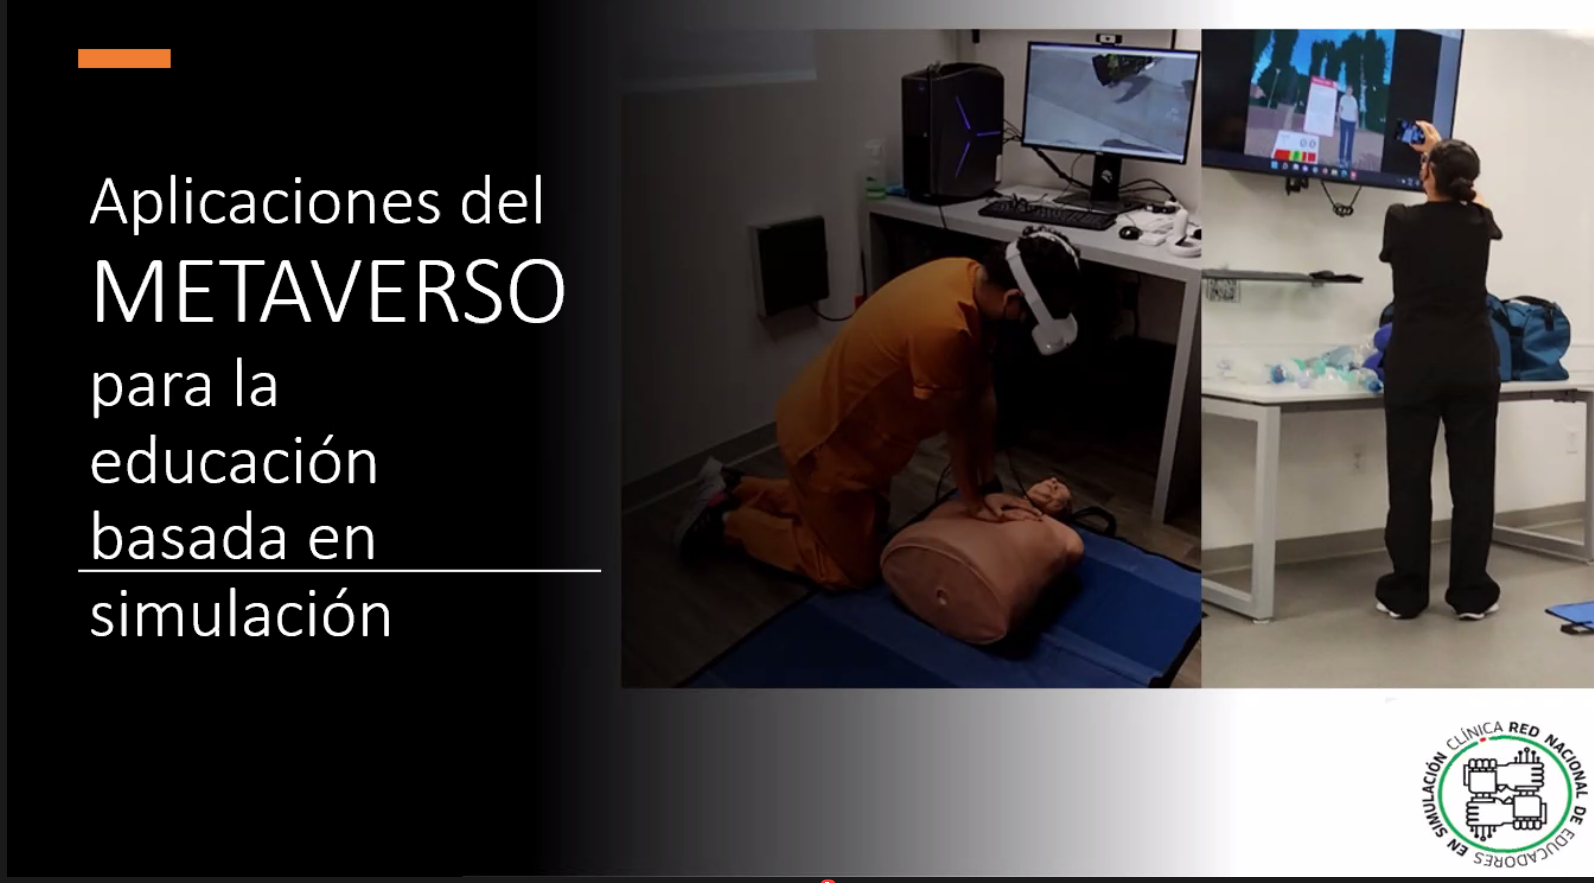
\includegraphics[width=8cm]{img_2}
 	\caption{Inicio de la conferencia con la Dra. Ariana Cerón}
 	\label{img_2}	
 \end{figure}

El metaverso compuesto por varias ramas de tecnología como es la realidad aumentada (RA), realidad virtual (RV) y en algunos casos la holografía. Estas ramas trataran de ser utilizadas para una mejor enseñanza práctica y sin riesgos que se acerque al mundo real (figura \ref{img_3})., ya que los médicos suelen aprender con personas reales, llegando a cometer equivocaciones que pueden ser fatales.

 	\begin{figure}[h]
	\centering
	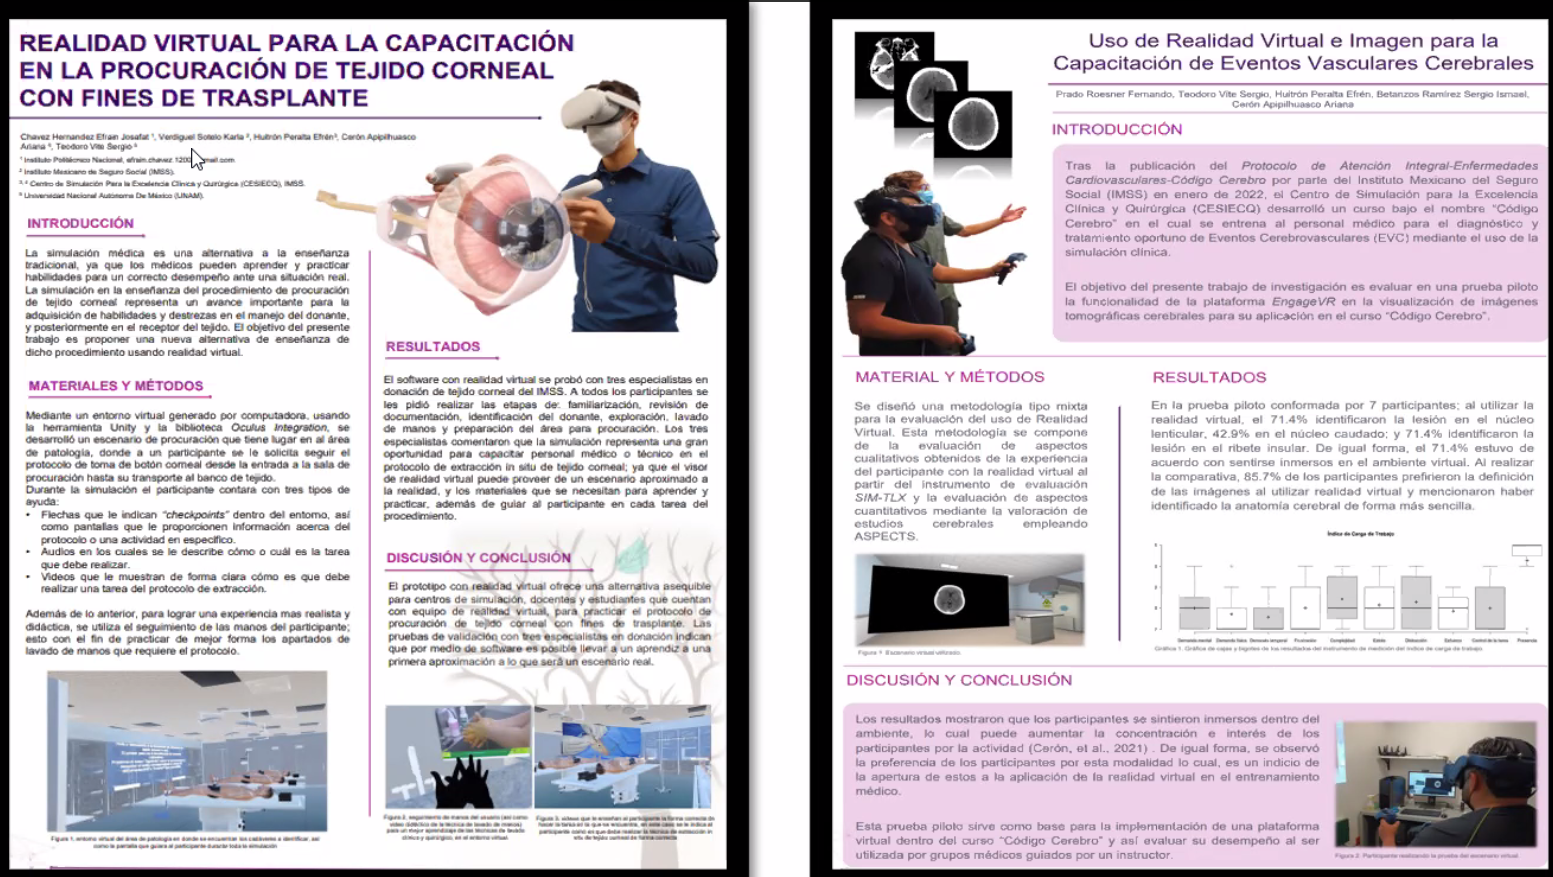
\includegraphics[width=14.3cm]{img_3}
	\caption{Proyectos realizados por el Centro de Simulación para la Excelencia Clínica y Quirúrgica del IMSS}
	\label{img_3}	
\end{figure}


    \section{Relación con la róbotica}
Este tipo de tecnología se usa de manera conjunta con sistemas robóticos para poder controlar lo que sucede dentro del metaverso, el navegar en el metaverso tendrá que ser igual que en el mundo real, para que eso suceda se tendrán que ocupar dispositivos para calcular los parámetros de nuestros movimientos. Y obviamente también se podrán diseñar robots en determinado momento para su uso dentro de este mismo mundo virtual. \\\vspace{0.1cm}

Se necesitará lo mencionado en la figura \ref{img_4} para seguir avanzando en este tipo de tecnología, ya que esta en sus inicios, su uso exponencial llevara algunos años. 

		\begin{figure}[h]
		\centering
		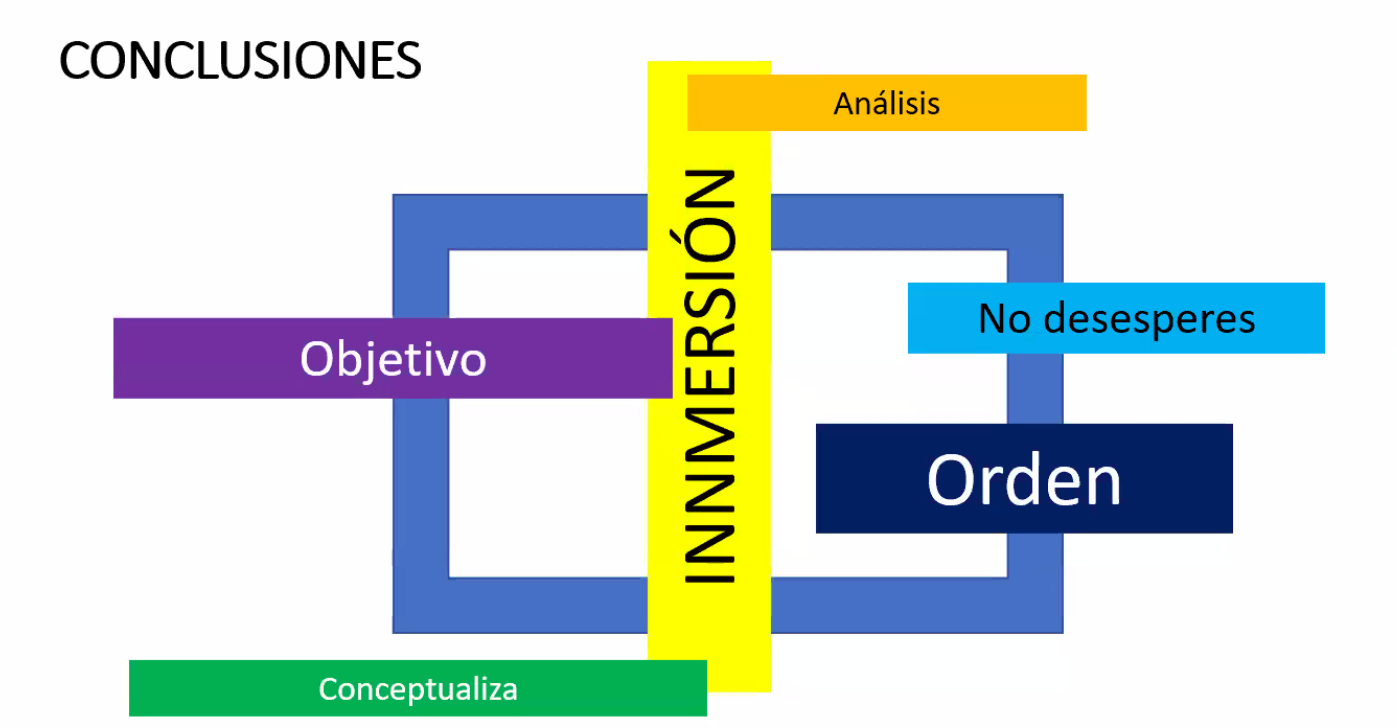
\includegraphics[width=15cm]{img_4}
		\caption{Conclusión de la conferencia}
		\label{img_4}	
	\end{figure}
		
 
	\end{document}